\chapter{Задача прямой кинематики} \label{ch:3}

\section{Введение} \label{sect3_1}
При разработке манипуляторов(и не только) возникает задача определения положения рабочего элемента по заданным углам. Данная проблема носит название "задача прямой кинематики". Решается с помощью простейших афинных преобразований, которые представляются в однородных координатах и матричной форме. Рассмотрим данный метод более подробно.

\section{Однородные координаты и матрицы преобразований}
Имея N-степеней свободы, мы можем представить операцию масштабирования и поворота с помощью матрицы размером $NxN$, в то же время мы не можем включить информацию о смещении. На помощь приходят однородные координаты, здесь к обычной матрице поворота(подразумеваем, что масштаб системы координат отдельных звеньев робота одинаков) добавляется столбец, включающий в себя смещение системы координат.

Например матрица:
\begin{align*}
	\begin{bmatrix}
		1	&	0				&	0				&	dx\\
		0	&	cos(\alpha)		&	-sin(\alpha)	&	dy\\
		0	&	sin(\alpha)		&	cos(\alpha)		&	dz\\
		0	&	0				&	0				&	1
	\end{bmatrix}
\end{align*}
не только поворачивает вектор вокруг оси $x$ на $\alpha$ градусов, но и смещает его на $dx$, $dy$, $dz$ вдоль осей $x$, $y$ и $z$ соответственно.

В качестве примера возьмем планарный трехзвенный механизм(см. рис. \ref{fig:ft_sheme1}). На изображении представлены звенья, их углы поворота и системы координат.
\begin{figure}[ht]
	\centering
	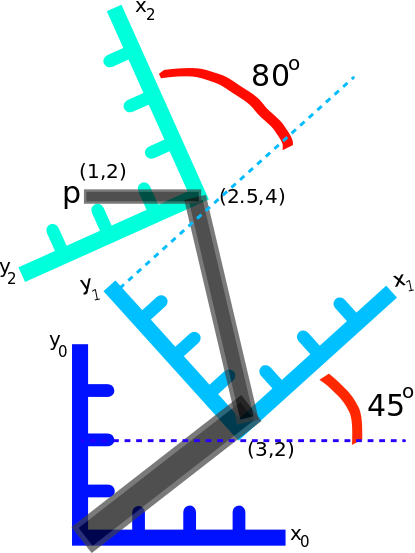
\includegraphics[scale=0.35]{FT/sheme1}
	\caption{Трехзвенный механизм и системы координат каждого звена}
	\label{fig:ft_sheme1}
\end{figure}



